\section{Smart spaces and middlewares}
\label{sec:smart_spaces}

Smart spaces are environments made up of different appliances that inter-work with each other and coordinate to proactively support the individuals in the environment for his/her daily activities. Smart spaces can refer to apartments, offices, museums, hospitals, schools, malls, university campuses and outdoor areas that are enabled for co-operation of smart objects and systems.

Mark Weiser envisioned smart spaces in 1991 as omnipresent computing devices spread out in the envirornmnet such that for humans their computing nature is oblivious \cite{Weiser1991}. He presented three technical requirements for the realization of smart spaces \cite{Weiser1991}\cite{pahl2014distributed}:

\begin{itemize}
  \item ``cheap, low-power computers that include equally convenient displays,''
  \item ``software for ubiquitous applications, and''
  \item ``a network that ties everything together''.
\end{itemize}

The vision of computers that interact with people's regular environments (``everyday's fabric'') is not reality in 2014 \cite{pahl2014distributed}. We present a short discussion on state of art by dividing the requirements under three items.

\subsection*{a. Devices}

Most smart devices are those that have wired or wireless network interfaces. Often used devices for household or office purposes are already available in the ``smart'' variants. Traditional non-smart devices have one specific purpose: fulfill the purpose of their utility in isolation. The newer appliances go beyond this by integrating extra computing units and network interfaces so they can be connected to a network. Smart devices in the professional and consumer domains are available and growing in their number 2014 \cite{pahl2014distributed}.

\begin{figure}
  \centering
  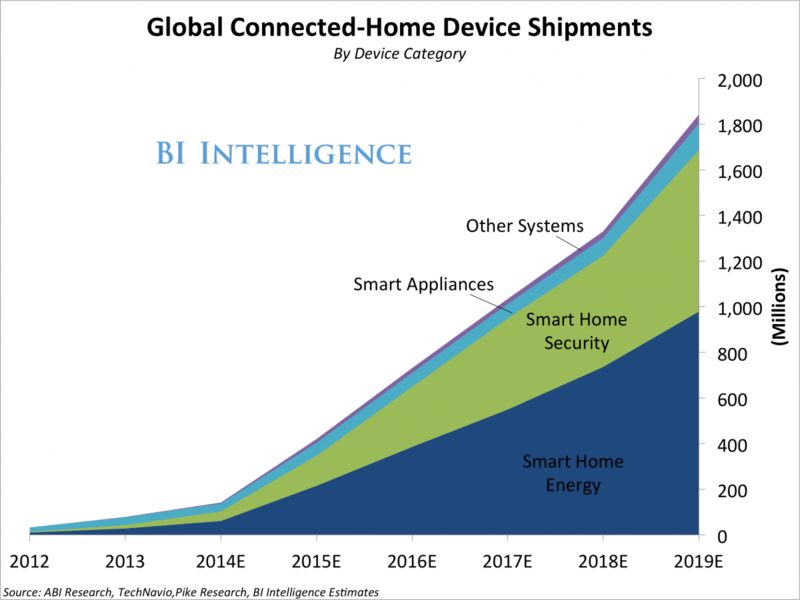
\includegraphics[width=10cm]{figures/connectedhomedevicecategories-1.png}
  \caption{Growth prediction of global connected home device shipments.}
  \label{fig:growth_home_device_with_categories}
\end{figure}

\subsection*{b. Networks}

In 2014, advancements in wired and wireless technologies have been achieved that allow sufficient bandwidth across short and long distance communications. WiFi technology is widely accepted to create networks in smaller spaces. Cellular networks provide highspeed connection to the Internet with third generation (3G) and fourth generation (4G) Long-Term Evolution (LTE) networks. Wireless networking standards like ZigBee, NFC, RFID and Bluetooth are used by small low powered digital radios \cite{warriach2013state}. Connectivity on physical level is already achieved. The challenge is to connect different types of devices (heterogeneous devices) on a semantic level \cite{pahl2014distributed}.

\subsection*{c. Softwares}

There already exists softwares that allow distributed computing. Technology like cloud-computing allows tasks to be divided and run in multiple computers. Software as a service (SAAS) providers have developed browser based applications for real time online collaboration across different types of devices. A part of the original vision has been achieved because we as humans have more advanced ways of collaborating with each other through computers. But computers have not disappeared into the background yet.

Softwares for pervasive computing have been a topic of wide research. These researches have focussed in different domains like health care and well being, e-Learning and campus life, tourism and traveling, office and other business applications, security and safety, energy saving, advertising and e-commerce, entertainment, user convenience, gaming, and social community applications \cite{pahl2014distributed}. When smart devices are managed via a software to create a smart space, it is called \emph{software orchestration}. Typically, the research projects implement software and hardware in exactly the same circumstances as the ones used during the research. The softwares that are produced are limited to their own domain and the domain environment, unsuitable for a different domain.

Marc-Oliver Pahl in his PhD dissertation described a new system called ``Distributed Smart Space Orchestration System (DS2OS)'' that presents a better approach of software orchestration \cite{pahl2014distributed}. DS2OS provides an open and portable middleware softare that can be used as a framework to develop new pervasive computing applications for wide variety of pervasive computing scenarios. DS2OS and its features are further described in Section \ref{sec:ds2os}.

\subsection*{Conclusion}

For all three requirements: devices, software and network already exists for pervasive computing scenario. The challenge is to build a platform that easily scales to the requirements of different domains and yet provides interoperability between them.

Further detailed state of the art for smart space middlewares and the networking technologies have been discussed in \cite{warriach2013state} and \cite{pahl2014distributed}.